\documentclass[12pt,table]{report}

\usepackage{amssymb}
\usepackage{amsmath}
\usepackage{fixlatvian}
\usepackage{polyglossia}
\usepackage{pgf}
\usepackage{subcaption}
\usepackage{graphicx}
\usepackage{geometry}
\usepackage{siunitx}
\usepackage[siunitx]{circuitikz}
\usepackage{floatrow}
\usepackage{pgfplots}
\usepackage{verbatim}
\usepackage{url}
\geometry{
 a4paper,
 total={170mm,257mm},
 left=20mm,
 top=20mm,
 bottom=20mm
}

\newfloatcommand{capbtabbox}{table}[][\FBwidth]

\title{1. laboratorijas darba atskaite}
\author{Jānis Ģeņģeris, REBM02}

\begin{document}
\maketitle

\chapter{Teorētiskā daļa}
\section{Ķēdes aprēķins}
Lai iegūtu sprieguma avota $V_1$ sprieguma vērtību voltos, jāizvēlas daļskaitlis,
kurš ir studenta apliecības pēdējo trīs ciparu dalījums ar 10. Lai iegūtu rezistor
$R_1$ vērtību, jāņem studenta apliecības priekšpēdējais cipars un tam jāpieskaita 1.
Līdzīgi iegūšt arī otra rezistora $R_2$ vērtību, taču šoreiz ņemot pēdejo studenta
apliecības numura ciparu, un pieskaitot tam 1. Mans studenta apliecības numurs ir
\emph{171REB166}, bet pēdējie 3 cipari ir $x=166$. Aprēķināsim $V_1$, $R_1$ un $R_2$
vērtības pēc iepriekš aprakstīta algoritma.

\begin{align}
V_1 = \frac{x}{10} = \frac{166}{10} &= \SI{16.6}{\volt}\,,\\
R_1 = \frac{\left(x \bmod 100\right)}{10} + 1
	= \frac{\left(166 \bmod 100\right)}{10} + 1 &= \SI{7}{\ohm}\,,\\
R_2 = \left(x \bmod 10\right) + 1 = \left(166 \bmod 10\right) + 1 &= \SI{7}{\ohm}\,.
\end{align}

Lai iegūtu spriegumu $U_{R_2}$ uz rezistora $R_2$, izmantosim
sprieguma dalītāja formulu \cite[43.lpp]{calexander2012}
\begin{equation}
U_{R_2} = V_1\cdot\frac{R_2}{R_1 + R_2} = 16.6\cdot \frac{7}{7 + 7} = \SI{8.3}{\volt}\,.
\end{equation}
Savukārt spriegumu $U_{R_1}$ iegūsim šādi
\begin{equation}
\label{eq:res_1}
U_{R_1} = V_1 - U_{R_2} = 16.6 - 8.3 = \SI{8.3}{\volt}\,.
\end{equation}
To pašu var iegūtu izmantojot Oma likumu \cite[30.lpp]{calexander2012}, lai iegūtu strāvu un pēc tam izrēķinot
sperigumus uz katra rezistora
\begin{equation}
\label{eq:res_2}
\begin{aligned}
I = \frac{U}{R_1 + R_2} = \frac{16.6}{14} &= \SI{1.186}{\ampere}\,,\\
U_{R_1} = R_1 \cdot I = 7 \cdot 1.186 &= \SI{8.302}{\volt}\,,\\
U_{R_2} = R_2 \cdot I = 7 \cdot 1.186 &= \SI{8.302}{\volt}\,.
\end{aligned}
\end{equation}
Redzams, ka (\nref{eq:res_2}) $U_{R_1}$ vērtība atšķiras no (\nref{eq:res_1}), par $\Delta=0.002$, kas
radies noapaļošanas kļūdu rezultātā.

\begin{figure}
\begin{floatrow}
\ffigbox{%
	\begin{circuitikz}[american voltages, american currents]
		\draw (0,3) to[american voltage source, v_=${V_1=\SI{16.6}{\volt}}$] (0,0);
		\draw (0,3) to[generic,l=${R_1=\SI{7}{\ohm}}$] (4,3);
		\draw (4,3) to[generic,l_=${R_2=\SI{7}{\ohm}}$] (4,0);
		\draw (0,0) to[short] (4,0);
	\end{circuitikz}
}{%
  \caption{Dotā ķēde.}%
	\label{fig:shema_01}
}
\capbtabbox{%
\begin{tabular}{|l|l|}
\hline
\rowcolor[HTML]{EFEFEF} 
Apzīmējums  & Vērtība          \\ \hline
$R_1$       & \SI{7}{\ohm}     \\ \hline
$R_2$       & \SI{7}{\ohm}     \\ \hline
$V_1$       & \SI{16.6}{\volt} \\ \hline
$U_{R_1}$   & \SI{8.3}{\volt}  \\ \hline
$U_{R_2}$   & \SI{8.3}{\volt}  \\ \hline
\end{tabular}
}{%
	\caption{Ķēdes elementu raksturlielumi.}
	\label{tab:elem_values}
}
\end{floatrow}
\end{figure}


\begin{figure}
\centering
\begin{tikzpicture}
\begin{axis}[
	width=0.8\textwidth,
	height=0.4\textwidth,
	grid=both,
	minor tick num=5,
	xmin=0,
	xmax=50,
	ymin=0,
	ymax=17,
	xlabel={$R_2$, $\Omega$},
	ylabel={$U_{R_2}$, \si{\volt}},
	legend pos=south east]
\addplot [orange, domain=0:50, very thick]{16.6*((x)/(7+x))};
\legend{$U_{R_2}=f(R_2)$}
\end{axis}
\end{tikzpicture}
\caption{$U_{R_2}$ atkarība no $R_2$.}
\end{figure}


\chapter{Praktiskā daļa}
\section{Darbs ar \emph{gEDA} programmām}
\subsection{Darbs ar \texttt{gschem}}

\begin{figure}[H]
\centering
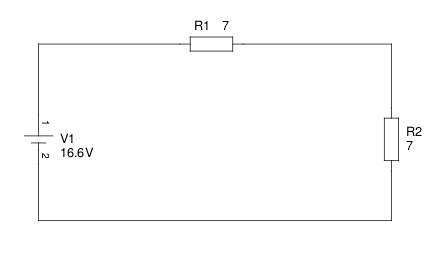
\includegraphics[scale=0.7]{img/gschem_1.png}
\caption{\emph{gschem} shēma \texttt{01.sch}.}
\label{att:shema_01}
\end{figure}


\subsection{Darbs ar \texttt{gnetlist}}
\begin{figure}[H]
\verbatiminput{01.net}
\caption{\emph{gnetlist} kods shēmai \texttt{01.sch}.}
\label{att:gnetlist_01}
\end{figure}

\subsection{Darbs ar \texttt{ngspice}}
\label{sec:darbs_ar_ngspice}
Attēlā nr. \nref{fig:r1_spriegums} redzams spriegums uz $R_1$ elementa, bet attēlā nr. \nref{fig:r2_spriegums} spriegums uz $R_2$
elementa. Savukārt attēlā \ref{fig:r1_r2_single} spriegums uz abiem elementiem vienā grafikā.

\begin{figure}[H]
    \centering
    \begin{subfigure}[b]{0.45\textwidth}
        \centering
				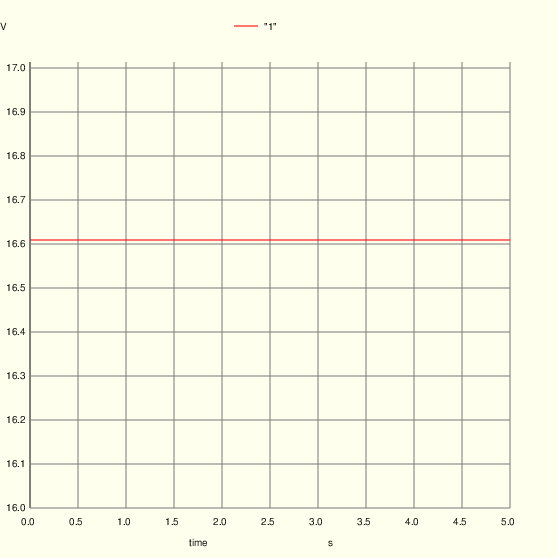
\includegraphics[scale=0.38]{img/plot1.png}
				\caption{Spriegums uz rezistora $R_1$.}
				\label{fig:r1_spriegums}
    \end{subfigure}%
    ~ 
    \begin{subfigure}[b]{0.45\textwidth}
        \centering
				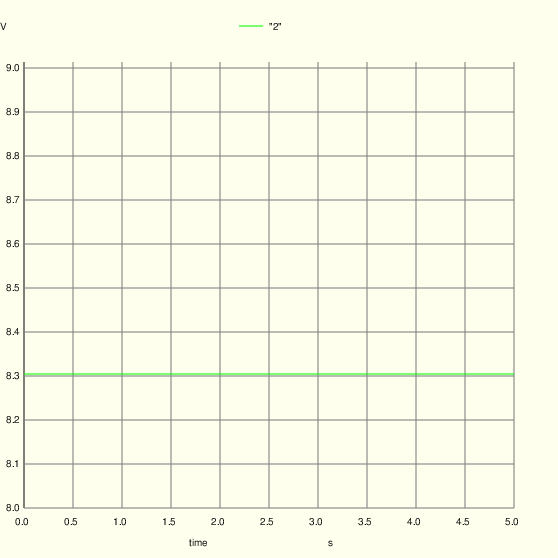
\includegraphics[scale=0.38]{img/plot2.png}
				\caption{Spriegums uz rezistora $R_2$.}
				\label{fig:r2_spriegums}
    \end{subfigure}
    \caption{Spriegums uz rezistoriem $R_1$ un $R_2$.}
\end{figure}

\begin{figure}[H]
    \centering
		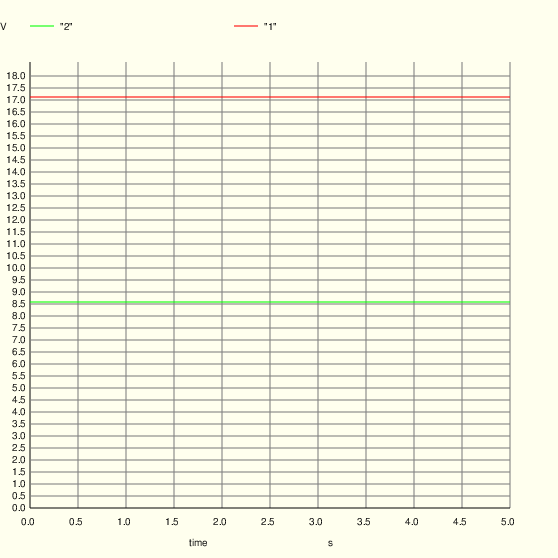
\includegraphics[width=0.45\textwidth]{img/plot3.png}
    \caption{Spriegums uz $R_1$ un $R_2$ vienā grafikā.}
    \label{fig:r1_r2_single}
\end{figure}

\section{Darbs ar \emph{QUCS} programmām}
\emph{QUCS} vidē tika izveidota \ref{fig:qucs_schem} attēlā redzamā shēma \emph{DC} un \emph{Sweep}
simulācijai. Šī shēma tika izmantota abām simulācijām, atbilstoši mainot parametra $x$ vērtības,
atkarībā no izvelētās simulācijas.

Lai iegūtu papildus informāciju darbam ar lineāru ķēžu simulācijām \emph{QUCS} vidē, lietderīgi izmantot
dokumnetāciju \cite{qucstutorial}.

\begin{figure}[H]
    \centering
		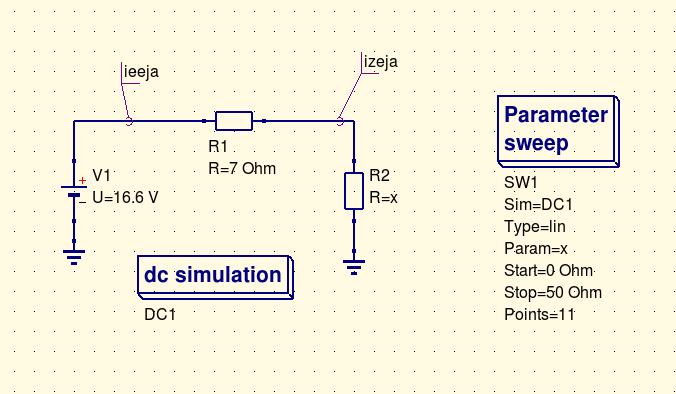
\includegraphics[width=0.6\textwidth]{img/qucs_schem.png}
    \caption{\emph{QUCS} simulācijas principālā shēma.}
    \label{fig:qucs_schem}
\end{figure}

\subsubsection{\emph{DC} simulācija}
Šeit izmantots konstantas rezistoru vērtības, no \ref{fig:qucs_dc} attēla redzams ka grafika
un tabulas vērtības ir konstantas uz abiem rezistoriem un tās sakrīt ar \emph{ngspice} simulācijas
rezultātiem sadaļā \nref{sec:darbs_ar_ngspice}.
\begin{figure}[H]
    \centering
		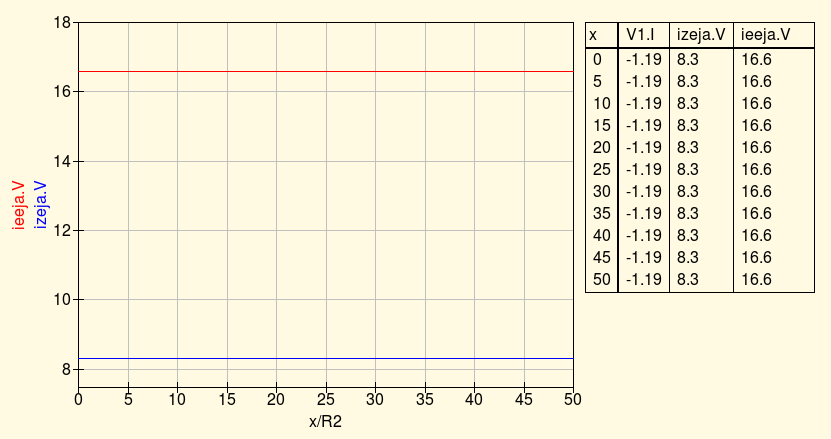
\includegraphics[width=0.6\textwidth]{img/qucs_simulation_dc.png}
    \caption{Līdzstrāvas simulācijas grafiks un tabula.}
    \label{fig:qucs_dc}
\end{figure}

\subsubsection{\emph{Sweep} simulācija}
Šeit izmantota mainīga rezistora $R_2$ vērtība (kurš apzīmēts ar $x$) intervālā no $0$ līdz $50$.
Rezultātā iegūts nelineārs grafiks kā tas labi redzams \ref{fig:qucs_sweep} attēlā un tabulā.
\begin{figure}[H]
    \centering
		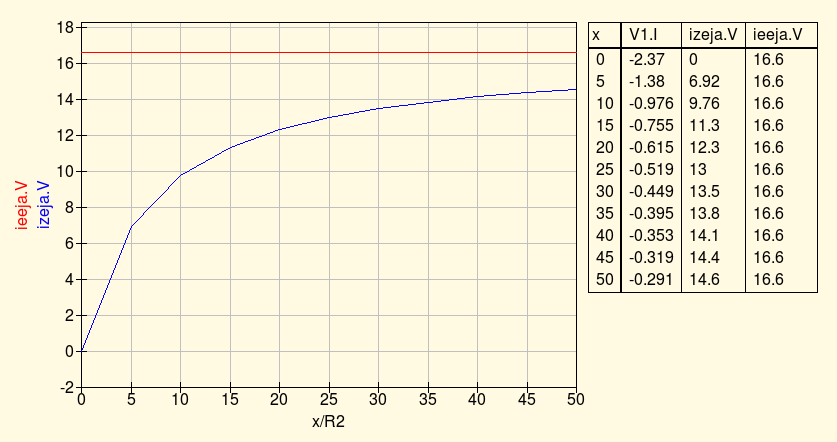
\includegraphics[width=0.6\textwidth]{img/qucs_simulation_sweep.png}
    \caption{\emph{Sweep} simulācijas grafiks un tabula.}
    \label{fig:qucs_sweep}
\end{figure}

\begin{thebibliography}{9}

\bibitem{calexander2012}
  Charles Alexander, Matthew Sadiku,
  Fundamentals of Electric Circuits
  McGraw-Hill Education,
  2th edition,
  2012.

\bibitem{pgfplotHelp}
  \emph{PGFPlots Gallery},
  \emph{PGFPlots} grafiku piemēri,
  \url{http://pgfplots.sourceforge.net/gallery.html},
  (\emph{pēdējā piekļūve 2018.05.23})

\bibitem{qucstutorial}
  Stefan Jahn, Chris Pitcher,
  DC Analysis, Parameter Sweep and Device Models, A Tutorial, Qucs,
  \url{http://qucs.sourceforge.net/docs/tutorial/dcstatic.pdf},
  2005,
  (\emph{pēdējā piekļūve 2018.05.23})

\end{thebibliography}

\end{document}
